\documentclass[margin=0px]{article}

\usepackage{listings}
\usepackage[utf8]{inputenc}
\usepackage{graphicx}
\usepackage{float}
\usepackage[a4paper, margin=1in]{geometry}
\usepackage{amsthm}
\usepackage{amssymb}

\renewcommand{\figurename}{ábra}
\makeatletter
\renewcommand\paragraph{%
	\@startsection{paragraph}{4}{0mm}%
	{-\baselineskip}%
	{.5\baselineskip}%
	{\normalfont\normalsize\bfseries}}
\makeatother
\renewcommand{\figurename}{ábra}
\newenvironment{tetel}[1]{\paragraph{#1}}{}
% A dokument itt kezdődik


\title{Záróvizsga tételsor \\ \large 10. Programnyelvi alapok}
\date{}
\author{Ancsin Ádám}

\begin{document}

	\maketitle
	
	\begin{tetel}{Programnyelvi alapok}
			Kifejezések kiértékelésének szabályai. Vezérlési szerkezetek: utasítások, rekurzió. Típusok: tömb, rekord, osztály, öröklődés, statikus és dinamikus kötés, polimorfizmus. Generikusok. Hatókör/láthatóság. Automatikus, statikus és dinamikus élettartam, szemétgyűjtés. Konstruktor, destruktor. Objektumok másolása, összehasonlítása. Alprogramok, paraméterátadás, túlterhelés.
	\end{tetel}
	
	\section{Kifejezések kiértékelésének szabályai}
	
	\noindent Fogalmak:
	\begin{itemize}
		\item	Operandusok: Változók, konstansok, függvény- és eljáráshívások.
		
		\item	Operátorok: Műveleti jelek, amelyek összekapcsolják egy kifejezésben az operandusokat és valamilyen
		műveletet jelölnek.
		
		\item	Kifejezés: operátorok és operandusok sorozata
		
		\item	Precedencia: A műveletek kiértékelési sorrendjét határozza meg.
		
		\item	Asszociativitás iránya: Az azonos precedenciájú operátorokat tartalmazó kifejezésekben a kiértékelés iránya.
		Megkülönböztetünk bal-asszociatív és jobb-asszociatív operátorokat.
	\end{itemize}
	
	\noindent Az operátorokat háromféleképpen írhatjuk az operandusokhoz képest:
	
	\begin{itemize}
		\item	Infix : Egy operátort a két operandusa közé kell írni (tehát csak kétoperandusú műveletek operátorait
		lehet így írni).
		Amikor egy kifejezésben több operátor is szerepel, akkor a különböző operátorok végrehajtási
		sorrendjét az operátorok precedenciája dönti el. Amelyik operátor precedenciája magasabb (pl. a
		szorzásé magasabb, mint az összeadásé), az általa jelölt műveletet értékeljük ki először. Ugyanazon
		operátorok végrehajtási sorrendjét pedig az asszociativitás iránya dönti el (pl. a bal-asszociatív azt
		jelenti, hogy balról jobbra haladva kell végrehajtani). Ezeket a (programozási nyelvekbe beépített)
		szabályokat zárójelek segítségével lehet felülírni.\\
		Példa: A * (B + C) / D
		
		\item	Postfix (Lengyelforma) : Az operátorokat az operandusaik mögé írjuk. A kiértékelés sorrendje mindig balról jobbra
		történik – tehát egy n operandusú operátor a tőle balra levő első n operandusra érvényes.\\
		Példa: A B C + * D /\\
		Ugyanez zárójelezve (felesleges): ((A (B C +) *) D /)
		
		\item	Prefix : Az operátorokat az operandusuk elé írjuk. A kiértékelés sorrendje balról
		jobbra történik.\\
		Példa: / * A + B C D\\
		Ugyanez zárójelezve (felesleges): (/ (* A (+ B C) ) D)\\
		Habár a prefix operátorok esetén is balról jobbra történik a kiértékelés, viszont ha egy operátortól
		jobbra egy másik operátor következik, akkor értelemszerűen az ehhez az operátorhoz tartozó
		műveletet kell először végrehajtani, hogy a bal oldalit is végre tudjuk hajtani. A fenti példában is a
		szorzást az osztás előtt, az összeadást pedig a szorzás előtt kell elvégezni.
	\end{itemize}
	
	\paragraph{Logikai operátorokat tartalmazó kifejezések kiértékelése}

	\noindent Az ilyen kifejezéseknek kétféle kiértékelése létezik:
	\begin{itemize}
		\item	Lusta kiértékelés : Ha az első argumentumból meghatározható a kifejezés értéke, akkor a másodikat
		már nem értékeli ki.
		\item	Mohó kiértékelés : Mindenféleképpen megállapítja mindkét argumentum logikai értékét.
	\end{itemize}	

	\noindent A két kiértékelési módszer bizonyos esetekben különböző eredményt adhat:
	\begin{itemize}
		\item	A 2. argumentum nem mindig értelmes\\
		Példa (C++): 
			\begin{verbatim}
			if ((i>=0) && (T[i]>=10))
			{
			    //...
			}
			\end{verbatim}
		Tegyük fel, hogy a T egy \texttt{int} tömb, 0-tól indexelődik.
		Itt ha az $i>=0$ hamis, akkor T-t alul indexelnénk. Ez mohó kiértékelés esetén futási idejű hibát okozna.
		Lusta kiértékelés esetén (a C++ alapértelmezetten ezt használja) viszont tudhatjuk, hogy a feltétel már nem lehet igaz, emiatt $T[i]>=10$-et már nem	kell kiértékelni.
		\item	A 2. argumentumnak van valamilyen mellékhatása.\\
	 	Példa (C++): 
			\begin{verbatim}
			if ((i>0) || (++j>0)) 
			{
			    T[j] = 100;
			}
			\end{verbatim}
		Ebben az esetben ha $i>0$ igaz, akkor a feltétel biztosan igaz, viszont a $++j>0$ kifejezés mellékhatásos, növeli j értékét.
		Mivel a C++ lusta kiértékelést használ a $||$ operátor esetén ($|$ operátor esetén mohó a kiértékelés), ezért ebben az esetben nem növeli j értékét. (csak akkor, ha $i>0$ hamis).
	\end{itemize}
	
	\section{Utasítások, vezérlési szerkezetek}
	
	\subsection{Egyszerű utasítások}
	
	\begin{itemize}
		\item	Értékadás : Az értékadás bal oldalán egy változó, a jobb oldalán bármilyen kifejezés állhat. Az
		értékadással a változóhoz rendeljük a jobb oldali kifejezést. Figyelni kell arra, hogy a bal oldali
		változó típusának megfelelő kifejezés álljon a jobb oldalon (vagy létezik implicit konverzió, pl. C++-ban
		az egész és logikai típus között). A legtöbb nyelvben az értékadás operátora az \texttt{=} (például C++, Java, C\#),
		vagy a \texttt{:=} (például Pascal, Ada).
	
		\item	Üres utasítás : Nem mindenhol lehet ilyet írni. A lényege, hogy nem csinál semmit.
		Azokban a nyelvekben lehet létjogosultsága,	ahol üres blokkot nem írhatunk,
		muszáj legalább 1 utasításnak szerepelnie benne. (pl. Ada) Erre szolgál az üres utasítás.
		(Ada-ban ez a \texttt{null} utasítás)
		
		\item	Alprogramhívás : Alprogramokat nevük és paramétereik megadásával hívhatunk.
		Példák: 
		\begin{itemize}
			\item	\texttt{System.out.println("Hello”);}
			\item	\texttt{int x = sum(3,4);}
		\end{itemize}
		\item	Visszatérés utasítás : Az utasítás hatására az alprogram végrehajtása befejeződik. Ha az alprogram egy
		függvény, akkor meg kell adni a visszatérési értéket is.
		
		\noindent Példák (C++): 
		\begin{itemize}
			\item	Ebben a példában a \texttt{doSomething} egy eljárás, nincs visszatérési értéke. A paraméterül kapott
			x változót értékül adjuk a j-nek. Ha ez az érték nem 0, akkor visszatérünk, azaz megszakítjuk az alprogram
			végrehajtását (konkrét értéket viszont nem adunk vissza). Ha ez az érték 0, akkor a végrehajtás folytatódik tovább,
			meghívjuk a \texttt{doSomethingElse} függvényt a j paraméterrel.
			\begin{verbatim}
			void doSomething(int x)
			{
			    int j;
			    if(j=x) 
			        return; // j!=0, do nothing
			
			    doSomethingElse(j);
			}
			\end{verbatim}
			
			\item Ebben a példában az \texttt{isOdd} egy függvény, \texttt{int} visszatérési értékkel. Megmondja a paraméterül kapott
			x egész számról, hogy páratlan-e. Ehhez bitenkénti ÉS művelettel "összeéseli" az x-et az 1-gyel (0...01). Ha az eredmény
			nem 0, akkor páratlan, visszatérünk igaz értékkel. Különben folytatjuk a működést, majd visszatérünk hamis értékkel. 
			\begin{verbatim}
			int isOdd(int x)
			{
			    if(x & 1) //bitwise AND with 0...01 is not 0...0
			        return true;
			        
			    return false;
			}
			\end{verbatim}
		\end{itemize}
		
		\item	Utasításblokk: A blokkon belüli utasítások "összetartoznak”.
		Ez több esetben is jól alkalmazható nyelvi elem:
		\begin{itemize}
			\item	Vezérlési szerkezetekben: Az adott vezérlési szerkezetekhez tartozó utasításokat különíthetjük el.

			\item	Az olyan nyelvekben, amelyekben deklaráció csak a program elején található deklarációs
			blokkokban lehetséges (pl. Ada), van lehetőség arra, hogy a programkód későbbi részében nyissunk
			egy blokkot, ahol deklarációk is szerepelhetnek.
			
			\item	Osztályok inicializáló blokkja pl. Java-ban (konstruktor előtt hajtódik végre):
			\begin{verbatim}
			public class MyClass{
			    private ResourceSet resourceSet;
			
			    {
			        resourceSet = new ResourceSetImpl();
			        UMLResourcesUtil.init(resourceSet);
			    }
			    
			    /* ...   */
			}
			\end{verbatim}
			\item	Osztályok statikus inicializáló blokkja pl. Java-ban:
			\begin{verbatim}
			public class MyClass{
			    private static ResourceSet resourceSet;
			    
			    static{
			        resourceSet = new ResourceSetImpl();
			        UMLResourcesUtil.init(resourceSet);
			    }
			    
			    /*  ...   */
			}
			\end{verbatim}
				
		\end{itemize}
	
	\end{itemize}

	\subsection{Vezérlési szerkezetek}
	
	\begin{itemize}
		\item	Elágazás : Az elágazás egy olyan vezérlési szerkezet, amellyel meghatározhatjuk, hogy bizonyos
		(blokkban megadott) utasítások csak a megadott feltétellel jöhessenek létre.
		Általában több feltételt is megadhatunk egymás után (if L1 then … else if L2 then … else if L3 then …).
		Megadhatjuk azt is, hogy mi történjen, ha egyik feltétel sem teljesül (if L then … else …).
	
		Elágazásokat lehet egymásba ágyazni (if … then if ...).
		
		"Csellengő else” ("Dangling else”) probléma: Azokban a nyelvekben lép fel, ahol egy feltétel egy
		utasításblokkját nem zárja le külön kódszó (pl. endif). Ekkor abban az esetben, ha elágazásokat
		egymásba ágyazunk, a következő probléma léphet fel:\\
		Példa: \texttt{if (A>B) then if (C>D) then E:=100; else F:=100;}
		
		A fenti esetben nem lehet megállapítani, hogy a programozó az else kulcsszót melyik elágazásra
		értette.
		
		\item	Ciklus : Egy utasításblokk (ciklusmag) valahányszori végrehajtását jelenti.
		\begin{itemize}
			\item	Feltétel nélküli ciklus : Végtelen ciklust kódol, kilépni belőle a strukturálatlan utasításokkal lehet
			(ld. lentebb), vagy return-nel, esetleg hiba fellépése esetén.
			
			Példa (ADA):
				\begin{verbatim}
					loop
					    null;
					end loop;
				\end{verbatim}
		
			\item	Elöltesztelő ciklus : A ciklus a ciklusmag minden végrehajtása előtt megvizsgálja, hogy az adott
			feltétel teljesül-e. Ha teljesül, akkor végrehajtja a magot, majd újra ellenőriz. Különben a ciklus
			után folytatódik a futás.
			
			Példák:
			\begin{itemize}
				\item	C++:
				\begin{verbatim}
					int x=0,y=0;
					while(x<5 && y<5)
					{
					    x+=y+1;
					    y=x-1;
					}
					cout<<x+y<<endl;
				\end{verbatim}
				
				\item	ADA:
				\begin{verbatim}
					declare
					    X,Y: Integer;
					begin
					    X:=0;
					    Y:=0;
					    while X<5 and Y<5 loop
					        X:=X+Y+1;
					        Y:=X-1;
					    end loop;
					end;
				\end{verbatim}
			\end{itemize}
			
			\item	Számlálásos ciklus : Ebben a vezérlési szerkezetben megadhatjuk, hogy a ciklusmag hányszor
			hajtódjon végre.
			Példa (ADA): 
			\begin{verbatim}
				for i in 1..10 loop 
				    null;
				end loop;
			\end{verbatim}
			A számlálás úgy történik, hogy egy változóban (ciklusváltozó) tároljuk, hogy "hol tartunk” - ezt hasonlítjuk
			össze minden ciklus elején a kifejezéssel, amit meg kell haladnia a változónak (i). Tehát
			felfogható egy elöltesztelő ciklusként is, ahol a ciklusfeltétel az \texttt{i<=10} és a ciklusmag végén
			növelni kell i-t.
			
			\item	Hátultesztelő ciklus : Az a különbség az elöltesztelőhöz képest, hogy a feltételt a ciklusmag
			végrehajtása után ellenőrizzük – tehát itt a ciklusmag 1-szer mindenképpen lefut.
			
			Példa (C++):
			
			\begin{verbatim}
				int i=0;
				do
				{
				    ++i;
				} while(i<5);
			\end{verbatim}
			
			Megjegyzés: vannak olyan nyelvek (pl. Pascal), amelyekben a hátultesztelő ciklus feltétele nem bennmaradási, hanem
			leállási feltétel. Azaz nem azt adjuk meg, hogy minek kell teljesülnie ahhoz, hogy még egyszer végrehajtásra kerüljön
			a ciklusmag, hanem azt, hogy minek kell teljesülnie ahhoz, hogy a ciklusmag ne hajtódjon végre többször.
			
			Az előbbi C++-os példa Pascal-os megfelelője:
			\begin{verbatim}
				i:=0;
				repeat
				    i:=i+1;
				until i=5;
			\end{verbatim}
			
			Megjegyzés: ADA-ban nincs igazi hátultesztelős ciklus. Ebben a nyelvben hátultesztelő ciklust úgy írhatunk, hogy ha
			írunk egy feltétel nélküli ciklust, amelynek utolsó utasítása egy feltételhez kötött kilépés.
			
			Példa:
			\begin{verbatim}
				i:=0;
				loop
				    i:=i+1;
				    exit when i=5;
				end loop;
			\end{verbatim}
			

			\item	foreach : Akkor használatos, ha egy adatszerkezet minden elemére végre akarjuk hajtani a magot.
			Tulajdonképpen ez is egy elöltesztelő ciklus (a ciklusfeltétel az, hogy a végére értünk-e az
			adatszerkezetnek).
			Példa: 
			\begin{verbatim}
				foreach (int v in Vect)
				{
				    ++v;
				}
			\end{verbatim}
			
			Megjegyzések: 
			\begin{enumerate}
				\item	Nincs minden programozási nyelvben ilyen ciklus. Leginkább az újabb nyelvekben terjedt el. 
				\item	Nem minden programozási nyelvben a foreach a kulcsszó ehhez a ciklushoz. 
				Például Java-ban, C++11-ben (régebbi változatokban nincs ilyen) a for ciklust használhatjuk foreach-ként:
				\begin{verbatim}
				int x=0;
				for (int v : vect){
				    x+=v;
				}
				\end{verbatim}
			\end{enumerate}

		\end{itemize}
	\end{itemize}

	\subsection{Strukturálatlan utasítások}
	
	\begin{itemize}
		\item	Ciklus megszakítása : A ciklusból való "kiugrásra” (tehát annak azonnali befejezésére) használható.
		Gyakran végtelen ciklus megszakítására használjuk, vagy hátultesztelő ciklus kódolására (ahol nincs
		erre beépített vezérlési szerkezet, például Ada).
	
		Ilyen utasítás pl. C/C++/C\#-ban, vagy Java-ban a \texttt{break}, illetve Ada-ban az \texttt{exit}.
		
		\item	\texttt{goto} utasítás : A programkódban címkéket definiálhatunk, majd a \texttt{goto} utasítással egy
		ilyen címkéhez irányíthatjuk a vezérlést. Vezérlési szerkezeteket is lehet vele kódolni. Túlzott
		használata olvashatatlan kódhoz vezethet.
	\end{itemize}
	
	\subsection{Rekurzió}
	
	Rekurzív alprogram: Olyan alprogram, amelynek kódjában szerepel önmagának a meghívása.
	Mindenképpen kell, hogy legyen a rekurziónak megállási feltétele – tehát egy olyan feltétel (egy elágazással
	együtt), amelynek teljesülése esetén nem történik rekurzív hívás, így az összes, folyamatban levő rekurzív hívás
	végre tud hajtódni (ellenkező esetben végtelen rekurzió lép fel, ilyenkor általában előbb-utóbb betelik a stack és leáll a program).\\
	
	\noindent Példák (faktoriális):
	
	\begin{itemize}
		\item	C++:
		\begin{verbatim}
			int fact (int n)
			{
			    if(n>0)
			        return n * fact (n-1);
			    else
			        return 1;
			}
		\end{verbatim}
		
		\item	Haskell:
		\begin{verbatim}
			fact :: (Integral a) => a -> a  
			fact n
			    | n>0 = n * fact (n - 1)  
			    | otherwise = 0
		\end{verbatim}
	
	\end{itemize}
	
	
	
	\section{Típusok}
	
	\subsection{Tömb}
	
	A tömb (angolul array) olyan adatszerkezet, amelyet nevesített elemek csoportja alkot, melyekre sorszámukkal (indexükkel) lehet hivatkozni. Vektornak is nevezik, ha egydimenziós, mátrixnak esetenként, ha többdimenziós. A legtöbb programozási nyelvben minden egyes elemnek azonos adattípusa van és a tömb folytonosan helyezkedik el a számítógép memóriájában. A készítés módja alapján lehet:
	
	\begin{itemize}
		\item	statikus :a méret fix, deklarációban szabályozott
		\item	dinamikus tömb: a mérete változik, folyamatosan bővíthető
	\end{itemize}

	\subsection{Rekord}
	
	A rekord egy összetett értékek leírásához használható konstrukció. Névvel és típussal ellátott összetevői vannak, ezeket mezőknek nevezzük.
	Értékhalmaz a mezők értéktípusai által meghatározott alaphalmazok direktszorzata.
	
	\begin{figure}[H]
		\centering
		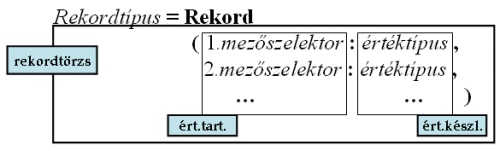
\includegraphics[width=0.7\linewidth]{img/rekord}
		\caption{A rekord-típuskonstrukciók általános szintaxisa.}
		\label{fig:rekord}
	\end{figure}
	
	\noindent Műveletek:
	\begin{itemize}
		\item	Szelekciós függvény (.mezőszelektor szintaxisú);
		
		\item	konstrukciós függvény (Rekordtípus(mezőértékek) szintaxisú);
		
		\item	elképzelhetők transzformációs függvények, amelyek a teljes rekordstruktúrát érintik.
	\end{itemize}
	
	\noindent Példa rekordra és használatára C-ben:
	\begin{verbatim}
	//definition of Point
	struct Point 
	{
	    int xCoord;
	    int yCoord;
	};
	
	const struct Point ORIGIN = {0,0};
	    
	\end{verbatim}
	
	\subsection{Osztály}
	
	Az osztály egy felhasználói típus, amelynek alapján példányok (objektumok)
	hozhatók létre. Az osztály alapvetően attribútum és metódus (művelet) definíciókat
	tartalmaz. Az osztály írja le az objektum típusát: megadja a tulajdonságait és azok
	lehetséges értékeit (azaz a típusértékeket), valamint az objektumon végrehajtható műveleteket (típusműveletek).\\
	
	\noindent Példa C++-ban:
	\begin{verbatim}
	//definition of Point
	class Point {
	private:
	    int xCoord;
	    int yCoord;
	public:
	    //constructor
	    Point(int xCoord, int yCoord) : xCoord(xCoord),yCoord(yCoord) {}
	    
	    void Translate(int dx, int dy) {
	        xCoord+=dx;
	        yCoord+=dy;
	    }
	    
	    void Translate(Point delta) {
	        xCoord+=delta.xCoord;
	        yCoord+=delta.yCoord;
	    }
	    
	    int getX() { return xCoord; }
	    
	    int getY() { return yCoord; }
	};
	
	int main(int argc, char* argv[])
	{
	    Point point(0,0);
	    point.Translate(5,-2);
	    cout<<point.getX()<<","<<point.getY()<<endl; //5,-2
	    Point delta(-2,1);
	    point.Translate(delta);
	    cout<<point.getX()<<","<<point.getY()<<endl; //3,-1
	    
	    return 0;
	}
	\end{verbatim}
	
	Megjegyzés: A nem objektum-orientált nyelvekben nincsenek osztályok, pl. régebbi nyelvekben, mint a C, ADA, Pascal, vagy
	funkcionális nyelvekben (Haskell, Clean, stb.).
	
	\subsection{Öröklődés}
	
	Egy osztály legegyszerűbben adattagjainak és metódusainak felsorolásával hozható létre. Azonban az objektum-orientált paradigma lehetőséget ad egy másik, hatékonyabb módszerre is, az öröklődésre. Az öröklődés az újrafelhasználhatóságot szem előtt tartva arra ad lehetőséget, hogy már meglévő (szülő-, ős-) osztályból kiindulva hozzunk létre új (gyermek-, leszármazott-, al-) osztályt. Az öröklés két osztály között fennálló olyan kapcsolat, amely során a leszármazott osztály rendelkezik a szülő osztály majdnem összes tulajdonságával (nem privát adattagjait és metódusait sajátjaként kezeli), s ezeket újabbakkal egészítheti ki. Az így létrehozott osztály is lehet más osztályok őse (kivéve pl. Java-ban a \texttt{final} kulcsszóval ellátott osztályok, ezekből már nem származtathatunk), így ezek az osztályok egy öröklési hierarchiába szerveződnek. Attól függően, hogy egy osztálynak egy- vagy több őse van, beszélünk egyszeres- ill. többszörös öröklődésről. A Java az egyszeres öröklődést támogatja, de pl. C++-ban van többszörös öröklődés.
	
	A Java-ban az osztályhierarchia legfelső eleme az Object osztály, amelyből minden más osztály (közvetve vagy közvetlenül) származik.
	
	Egy alosztály az örökölt metódusokat újraimplementálhatja. Ilyenkor az adott metódus ugyanolyan néven, de más, módosított (alosztályra specifikált) tartalommal kerül megvalósításra. Az ilyen metódusokat polimorfnak nevezzük. Java-ban minden olyan metódust, ami nincs ellátva a \texttt{final} kulcsszóval, újra lehet definiálni. (C++-ban mindent, ami nem privát)\\
	
	\noindent Példák:
	\begin{itemize}
		\item	C++:
		\begin{verbatim}
		    class RegularPolygon
		    {
		    protected:
		        const double radius;
		    public:
		        RegularPolygon(double radius) : radius(radius) {}
		        virtual double area() = 0;
		    };
		    
		    class EquilateralTriangle : public RegularPolygon
		    {
		    public:
		        EquilateralTriangle(double radius) : RegularPolygon(radius) {}
		        virtual double area()
		        {
		             return 0.75*sqrt(3.0)*radius*radius;
		        }
		    };
		\end{verbatim}
		
		\item	Java:
		\begin{verbatim}
		public abstract class RegularPolygon{
		    protected final double radius;
		
		    public RegularPolygon(double radius){
		        this.radius = radius;
		    }
		    public abstract double area();
		}
		
		public class EquilateralTriangle extends RegularPolygon{
		    public EquilateralTriangle(double radius){
		        super(radius);
		    }
		    public double area(){
	 	        return 0.75*Math.sqrt(3.0)*radius*radius;
		    }
		}
		
		\end{verbatim}
	\end{itemize}
	
	\subsection{Statikus és dinamikus kötés}
	
	\begin{itemize}
		\item	statikus típus: A változó deklarációjában megadott típus. Fordítás során egyértelműen eldől, nem változhat
		futás során. A statikus típus határozza meg, hogy mit szabad csinálni az objektummal (pl. hogy milyen
		műveletek hívhatók meg rá).
		
		\item	dinamikus típus: A változó által hivatkozott objektum típusa. Vagy a statikus típus leszármazottja, vagy maga
		a statikus típus. Futás során változhat.
	\end{itemize}
	
	\noindent Példa(Java):
	\begin{verbatim}
		Object o = new String("Hello”);
	\end{verbatim} 
	Itt az o változó statikus típusa \texttt{Object}, dinamikus típusa pedig \texttt{String}.\\

	\noindent Kötések:
	\begin{itemize}
		\item	statikus kötés: A változó statikus típusa szerinti adattagokra lehet hivatkozni.
		\item	dinamikus kötés: A változó dinamikus típusa szerinti adattagok használhatók.
	\end{itemize}
	
	A kötés akkor fontos, ha a hívott művelet, vagy a hivatkozott változó a statikus és a dinamikus típusban
	különbözik, vagy esetleg a statikus típusban nem is létezik (ekkor a dinamikus típusban sem hivatkozhatunk
	az adattagra).\\

	\noindent Többféleképpen lehet a kötéseket meghatározni a különböző nyelvekben:
	\begin{itemize}
		\item	Java : Minden esetben dinamikus kötés van (az örökölt metódusok törzsében is).
		\item	C++ : A művelet definiálásakor lehet jelezni, ha dinamikus kötést szeretnénk (\texttt{virtual}).
		\item	Ada : A híváskor lehet jelezni, ha dinamikus kötést szeretnénk.
	\end{itemize}

	
	\section{Generikusok}
	
	Generikus programozás: Algoritmusok, adatszerkezetek általánosított, több típusra is működő
	leprogramozása (pl. generikus rendezés, generikus verem, …). Ezt az általános kódot nevezzük sablonnak
	(template).
	
	Bizonyos nyelvekben (Ada, C++) egy sablont példányosítani kell – ekkor a kívánt típusokat, objektumokat
	(a sablon definíciónak megfelelően) a sablonnak paraméterként megadva példányosul a szóban forgó sablon.
	(Ugyanúgy, mint pl. amikor egy függvénynek megadjuk az aktuális paraméterét.) Ezt nevezzük generatív
	programozásnak: a program a megadott sablon alapján létrehoz egy "igazi” programegységet (program
	generál programot).
	
	Példa: Egy verem sablon példányosításakor megadjuk, hogy milyen típusú elemeket tároljon a verem (típus
	paraméter) és hogy hány elem fér a verembe (objektum paraméter).
	C++ és Ada esetén egy sablon paramétere alprogram is lehet.
		
	Példa: Egy rendezésnek megadjuk, hogy milyen művelet alapján rendezzen.
	Természetesen lehet alapértelmezett sablonparaméter is.
	
	Egy sablon definiálása esetén természetesen a sablont nem lehet minden típusra használni. Egy sablon attól
	lesz sablon, hogy több típusra is működik. Azonban megszorításokat tehetünk (és tennünk is kell) arra, hogy
	milyen típusokra lehessen azt használni, hogyan lehessen a sablont példányosítani.

	Jó példa erre az Ada nyelv, ahol a sablon specifikációja egy "szerződés” a sablon törzse és a példányosítás
	között:
	
	\begin{itemize}
		\item	A sablon törzse nem használhat mást, csak amit a sablon specifikációja megenged neki. (A törzset
		nem feltétlenül kell, hogy ismerjük példányosításkor.)
		\begin{verbatim}
			generic
			    type Element_T is private;
			    with function "*" (X, Y: Element_T) return Element_T is <>;
			function Square (X : Element_T) return Element_T;
		\end{verbatim}
		Itt a \texttt{with function} kezdetű sor végén az \texttt{is <>} azt jelenti, hogy ha az adott típusra már létezik *
		művelet (pl. egész számokra), akkor nem kell külön megadni példányosításkor, a program automatikusan azt használja.
		
		A törzs:
		\begin{verbatim}
			function Square (X: Element_T) return Element_T is
			begin
			    return X * X;   -- The formal operator "*".
			end Square;
		\end{verbatim}
		
		\item	A példányosításnak biztosítania kell mindent, amit a sablon specifikációja megkövetel tőle.
		A következő példában a négyzetre emelő függvényt mátrixokra alkalmazzuk, feltéve, hogy definiáltuk a
		mátrixszorzást.
		\begin{verbatim}
			with Square;
			with Matrices;
			procedure Matrix_Example is
			    function Square_Matrix is new Square
			        (Element_T => Matrices.Matrix_T, "*" => Matrices.Product);
			    A : Matrices.Matrix_T := Matrices.Identity;
			begin
			    A := Square_Matrix (A);
			end Matrix_Example;
		\end{verbatim}
	\end{itemize}

	Például a C++-ban a sablonszerződés nem így működik. Ott a sablon specifikációja az egész
	definíció (emiatt sablonosztályokat csak teljes egészében header fájlokban definiálhatunk).
	Példányosításkor ezt is ismerni kell, hogy tudjuk, hogyan példányosíthatunk. Az információelrejtés
	elve tehát sérül.
	
	Más nyelvekben (pl. Java, funkcionális nyelvek) nem kell a sablonokat példányosítani – mindig ugyanaz a
	megírt kód hajtódik végre, csak épp az aktuális paraméterekkel. Pl. Java-ban a típusparaméter fordításkor "elveszik",
	csak futási időben derül ki.
	
	\section{Hatókör/láthatóság}
	
	\begin{enumerate}
		\item	Hatókör: Deklarációkor a programozó összekapcsol egy entitást (például egy változót vagy függvényt) egy névvel. A hatókör alatt a forrásszöveg azt a részét értjük, amíg ez az összekapcsolás érvényben van. Ez általában annak a blokknak a végéig tart, amely tartalmazza az adott deklarációt.
		
		\item	A láthatóság a hatókör részhalmaza, a programszöveg azon része, ahol a deklarált névhez a megadott entitás tartozik. Mivel az egymásba ágyazott blokkokban egy korábban már bevezetett nevet más entitáshoz kapcsolhatunk, ezért ilyenkor a külső blokkban deklarált entitás a nevével már nem elérhető. Ezt nevezzük a láthatóság elfedésének.
		
		Egyes nyelvekben (például C++) bizonyos esetekben (például osztályszintű adattagok) a külső blokkban deklarált entitáshoz minősített névvel hozzá lehet férni ekkor is.
	\end{enumerate}
	
	\section{Automatikus, statikus és dinamikus élettartam, szemétgyűjtés}
	Élettartam: A változók élettartama alatt a program végrehajtási idejének azt a szakaszát értjük, amíg a változó számára lefoglalt tárhely a változóé.
	
	\subsection{Automatikus élettartam}
	
	A blokkokban deklarált lokális változók automatikus élettartamúak, ami azt jelenti, hogy a deklarációtól a tartalmazó blokk végéig tart, azaz egybeesik a hatókörrel. A helyfoglalás számukra a végrehajtási verem aktuális aktivációs rekordjában történik meg.
	
	\subsection{Statikus élettartam}
	
	A globális változók, illetve egyes nyelvekben a statikusként deklarált változók (például C/C++ esetén a \texttt{static} kulcsszóval) statikus élettartamúak. Az ilyen változók élettartama a program teljes végrehajtási idejére kiterjed, számukra a helyfoglalás már a fordítási időben megtörténhet.
	
	\subsection{Dinamikus élettartam}
	
	A dinamikus élettartamú változók esetén a programozó foglal helyet számukra a dinamikus tárterületen (heap), és a programozó feladata gondoskodni arról is, hogy ezt a tárterületet később felszabadítsa. Amennyiben utóbbiról megfeledkezik, azt nevezzük memóriaszivárgásnak (memory leak).
	Mint látjuk, a dinamikus élettartam esetén a hatókör semmilyen módon nem kapcsolódik össze az élettartammal, az élettartam szűkebb vagy tágabb is lehet a hatókörnél.
	
	\subsection{Szemétgyűjtő}
	
	A szemétgyűjtő másik neve a hulladékgyűjtő, az angol Garbage Collector név után pedig gyakran csak GC-nek rövidítik. Feladata a dinamikus memóriakezeléshez kapcsolódó tárhelyfelszabadítás automatizálása, és a felelősség levétele a programozó válláról, így csökkentve a hibalehetőséget.
	
	A szemétgyűjtő figyeli, hogy mely változók kerültek ki a hatókörükből, és azokat felszabadíthatóvá nyilvánítja. A módszer hátránya a számításigényessége, illetve a nemdeterminisztikussága. A szemétgyűjtő ugyanis nem szabadítja fel egyből a hatókörükből kikerült változókat, és a felszabadítás sorrendje sem ugyanaz, amilyen sorrendben a változók felszabadíthatóvá váltak.
	
	Azt, hogy a hulladékgyűjtő mikor és mely változót szabadítja fel, egy programozási nyelvenként egyedi, összetett algoritmus határozza meg, amelyben rendszerint szerepet játszik a rendelkezésre álló memória telítettsége, illetve a felszabadításhoz szükséges becsült idő. (Például ha egy objektum rendelkezik destruktorral, akkor általában a GC később szabadítja csak fel.)
	
	Összességében a szemétgyűjtő csak annyit garantál, hogy előbb-utóbb (legkésőbb a program futásának végeztével) minden dinamikusan allokált változót felszabadít.
	
	Szemétgyűjtést használó nyelvek pl. Java, C\#, Ada. C/C++-ban nincs szemétgyűjtés, a programozónak kell gondoskodni a dinamikusan allokált memóriaterületek felszabadításáról.
	\section{Konstruktor, destruktor}

	\subsection{Konstruktor}
	
	A konstruktor az objektumok inicializáló eljárása, akkor fut le, ha egy osztályból új objektumot példányosítunk. Alapértelmezett konstruktor alatt a paraméter nélküli konstruktort értjük, a legtöbb programozási nyelv esetén ezt a fordítóprogram automatikusan generálja üres törzzsel, amennyiben nem lett megadva egy konstruktor sem egy osztályban.
	Többek között a konstruktorban szokás gondoskodni arról, hogy az objektum dinamikus élettartamú változói számára tárhelyet foglaljunk.
	
	\subsection{Destruktor}
	
	A destruktor a konstruktor ellentétes párja, ez az eljárás az objektumok felszabadításakor fut le. Meghívása automatikusan megtörténik, attól függetlenül, hogy az objektum felszabadítása automatikusan történik a hatókör végeztével (lokális objektumok esetén), manuálisan a programozó	által (dinamikus élettartamú objektumok esetén) vagy a szemétgyűjtő által (szintén dinamikus élettartamú objektumok esetén).
	
	A desktruktorban szokás többek között az objektum dinamikus helyfoglalású adattagjait és a lefoglalt erőforrásokat felszabadítani.
	
	\section{Objektumok másolása, összehasonlítása}
	
	Az objektumok másolása egy speciális konstruktorral, az úgynevezett másoló konstruktorral (copy constructor) történik. Ez paraméterül az adott osztály egy példányát kapja meg, és azt a programozó által megadott működési logika szerint lemásolja az éppen inicializált objektumba.
	
	Több programozási nyelv (például C++) fordítóprogramja automatikusan elkészít egy másoló konstruktort, ha a programozó nem definiál sajátot. Ez az alapértelmezett másoló konstruktor lemásolja a forrásobjektum összes adattagjának értékét, ezt nevezzük sekély másolatnak (shallow copy). Ha az objektum dinamikus foglalású adattagokat is tartalmaz, akkor azoknak nem az értéke, hanem csak a hivatkozása lesz lemásolva, ami általában nem a kívánt működés. Ez esetben saját másoló konstruktor írása szükséges, ami mély másolatot (deep copy) készít.
	
	\section{Alprogramok, paraméterátadás, túlterhelés}
	
	\subsection{Alprogramok}
	
	Alprogramoknak a függvényeket, eljárásokat és műveleteket nevezzük. Segítségükkel a program feladatonként tagolható, a főprogramból az önálló feladatok kiszervezhetőek.
	
	\subsection{Paraméterátadás}
	
	Az alprogramoknak szüksége lehet bemenő adatokra és vissza is adhat értékeket. Az alprogramokat általános írjuk meg, saját változónevekkel, ezek a formális paraméterek. Az alprogram meghívásakor az átadott aktuális paraméterek alapján a formális paraméterek értéket kapnak. Az, hogy a formális paraméterek értéke mi lesz, a paraméterátadás módjától függ.
	
	\subsubsection{Szövegszerű paraméterátadás}
	
	A makrókban használatosak mind a mai napig. A makró törzsében a formális paraméter helyére beíródik az aktuális paraméter szövege.
	
	\subsubsection{Név szerinti paraméterátadás}
	
	Az aktuális paraméter kifejezést újra és újra kiértékeljük, ahányszor hivatkozás történik a formálisra. A paramétert a törzs kontextusában értékeljük ki, így a formális paraméter különböző előfordulásai mást és mást jelenthetnek az alprogramon belül.
	Alkalmazása archaikus (például: Algol 60, Simula 67).
	
	\subsubsection{Érték szerinti paraméterátadás}
	
	Az egyik legelterjedtebb paraméterátadási mód (például: C, C++, Pascal, Ada, Java), bemeneti szemantikájú. A formális paraméter az alprogram lokális változója, híváskor a vermen készül egy másolat az aktuális paraméterről, ez lesz a formális. Az alprogram végén a formális paraméter megszűnik
	
	\subsubsection{Cím szerinti paraméterátadás}
	
	A másik legelterjedtebb paraméterátadási mód (például: Pascal, C++, C\#), be- és kimeneti szemantikájú. A híváskor az aktuális paraméter címe adódik át, azaz a formális és az aktuális paraméter ugyanazt az objektumot jelentik, egy alias jön létre.\\
	
	Megjegyzés: A Java-ban nincs cím szerinti paraméterátadás, csak érték szerinti. A Java ugyanis a primitív típusoknak az értékét tárolja,
	objektumok esetén pedig egy referenciát az adott objektumra (mint C++-ban a referencia típus).  Objektum átadásakor ez a referencia másolódik le, azaz a referencia adódik át érték szerint.\\
	
	\noindent	Például:
	\begin{verbatim}
	    public static void BadSwap(Object x, Object y)
	    {
	        Object tmp = x;
	        x = y;
	        y = tmp;
	    }
	\end{verbatim}
	
	A fenti függvény nem cseréli ki az x-et és y-t, csak lokálisan (a függvénytörzsön belül), viszont a hívás helyén
	x és y is helyben maradnak.
	
	\subsubsection{Eredmény szerinti paraméterátadás}
	
	Kimeneti szemantikájú paraméterátadási mód. A formális paraméter az alprogram lokális változója, az alprogram végén a formális paraméter értéke bemásolódik az aktuálisba. Azonban az alprogram meghívásakor az aktuális értéke nem másolódik be a formálisba. (Használja például az Ada.)
	
	\subsubsection{Érték/eredmény szerinti paraméterátadás}
	
	Az érték és eredmény szerinti paraméterátadás összekombinálása, így egy be- és kimeneti szemantikájú paraméterátadási módot kapunk. (Használja például az Algol-W vagy az Ada.)
	
	\subsubsection{Megosztás szerinti paraméterátadás}
	
	Objektumorientált programozási nyelvek (például: CLU, Eiffel) paraméterátadási módja. Lényege, hogy ha a formális paraméter megváltoztatható és az aktuális paraméter egy megváltoztatható változó, akkor cím szerinti paraméterátadás történik, egyébként pedig érték szerinti. A paraméterátadás módját külön megadni nem lehet.
	Megváltoztatható (mutable) objektum alatt azt értjük, hogy tulajdonságai, ezáltal állapota megváltoztatható.
	
	\subsubsection{Igény szerinti paraméterátadás}
	
	Ezt a paraméterátadási módot a lusta kiértékelésű funkcionális nyelvek (például: Clean, Haskell, Miranda) alkalmazzák. Az aktuális paramétert nem híváskor értékeli ki, hanem akkor, amikor először szüksége van rá a számításokhoz.
	
	\subsection{Túlterhelés}
	
	A túlterhelés (overloading) segítségével azonos nevű alprogramokat hozhatunk létre eltérő szignatúrával. A szignatúra a legtöbb programozási nyelvben az alprogram nevét és a formális paraméterek számát és típusát jelenti, de egyes nyelvekben (például Ada) a visszatérési érték típusa is beletartozik. A túlterhelés elsődleges felhasználási területe, hogy ugyanazt a tevékenységet különböző paraméterezéssel is elvégezhessük.
	
	A fordító az alprogramhívásból el tudja dönteni, hogy a túlterhelt változatok közül melyiket kell meghívni. Ha egyik sem illeszkedik vagy több is illeszkedik, akkor fordítási hiba lép fel.
	
\end{document}